\documentclass[10pt]{article}

\usepackage[margin=0.55in]{geometry}
\usepackage[T1]{fontenc}
\usepackage[utf8]{inputenc}
\usepackage{lmodern}
\usepackage{microtype}
\usepackage{graphicx}
\usepackage{tikz}
\usepackage{pgfplots}
\usepackage{xcolor}
\usepackage{caption}
\usepackage{hyperref}

\usetikzlibrary{
  arrows.meta,
  backgrounds,
  calc,
  decorations.pathreplacing,
  fit,
  matrix,
  positioning,
  shadows,
  shapes.geometric
}
\pgfplotsset{compat=1.18}

\definecolor{grondInk}{HTML}{17212B}
\definecolor{grondMuted}{HTML}{5A6673}
\definecolor{grondBlue}{HTML}{276EF1}
\definecolor{grondCyan}{HTML}{11A7B5}
\definecolor{grondGreen}{HTML}{2E9D63}
\definecolor{grondAmber}{HTML}{D88A1D}
\definecolor{grondRed}{HTML}{B94444}
\definecolor{grondViolet}{HTML}{7657D6}
\definecolor{grondPaper}{HTML}{F7F8FA}
\definecolor{grondLine}{HTML}{D7DEE8}

\hypersetup{
  colorlinks=true,
  linkcolor=grondBlue,
  urlcolor=grondBlue
}

\captionsetup{
  font={sf,small},
  labelfont={bf},
  justification=raggedright,
  singlelinecheck=false
}

\tikzset{
  flow/.style={-Latex, line width=0.95pt, draw=grondInk!72},
  softflow/.style={-Latex, line width=0.75pt, draw=grondMuted!70},
  gateflow/.style={-Latex, line width=0.9pt, draw=grondAmber!88},
  rejectflow/.style={-Latex, line width=0.9pt, draw=grondRed!80, dashed},
  box/.style={
    rounded corners=5pt,
    draw=grondLine,
    line width=0.9pt,
    fill=white,
    text=grondInk,
    align=center,
    font=\sffamily\small,
    inner sep=5pt,
    minimum height=12mm,
    drop shadow={shadow xshift=0.7pt, shadow yshift=-0.7pt, opacity=0.12}
  },
  inputbox/.style={box, fill=grondBlue!7, draw=grondBlue!35},
  enginebox/.style={box, fill=grondCyan!7, draw=grondCyan!45},
  updatebox/.style={box, fill=grondViolet!7, draw=grondViolet!45},
  outputbox/.style={box, fill=grondGreen!8, draw=grondGreen!45},
  riskbox/.style={box, fill=grondAmber!10, draw=grondAmber!55},
  stopbox/.style={box, fill=grondRed!8, draw=grondRed!45},
  smallbox/.style={box, font=\sffamily\scriptsize, minimum height=9mm, inner sep=4pt},
  decision/.style={
    diamond,
    aspect=2.15,
    draw=grondAmber!72,
    fill=grondAmber!10,
    line width=0.9pt,
    align=center,
    font=\sffamily\scriptsize,
    inner sep=1.5pt,
    text=grondInk,
    drop shadow={shadow xshift=0.6pt, shadow yshift=-0.6pt, opacity=0.10}
  },
  lane/.style={
    rounded corners=7pt,
    draw=grondLine,
    fill=grondPaper,
    line width=0.8pt
  },
  stage/.style={font=\sffamily\bfseries\large, text=grondInk},
  note/.style={font=\sffamily\scriptsize, text=grondMuted, align=center},
  tag/.style={
    rounded corners=3pt,
    fill=grondInk!6,
    draw=grondInk!14,
    font=\sffamily\scriptsize,
    text=grondMuted,
    inner sep=3pt
  }
}

\newcommand{\grondTitle}[1]{%
  \vspace*{-2mm}
  {\sffamily\bfseries\Large\color{grondInk}#1}\par\vspace{2mm}
}

\newcommand{\grondSub}[1]{%
  {\sffamily\small\color{grondMuted}#1}\par\vspace{4mm}
}

\title{\sffamily\bfseries GROND Workflow Figures}
\author{\sffamily Global Regularization Of Non-kinematical Diffraction}
\date{}

\begin{document}
\maketitle
\thispagestyle{empty}

\section*{Figure Set}
These figures describe how GROND takes a reintegrated XDS directory plus a solved
structure and turns row-level observations into Bloch/Born predictions, corrected
reflection files, endpoint statistics, forensic audits, and maps. The diagrams
are written as source figures for papers, talks, and lab documentation. For a
non-expert reader, a \emph{row} means one measured spot observation from the
integration table. A \emph{merged reflection} means several rows have already
been combined. GROND keeps rows alive for as long as possible because row-level
geometry, thickness, polarity, and weak-reflection behavior are where many useful
diagnostics live.

\clearpage

\begin{figure}[p]
\centering
\grondTitle{Overall GROND Operating Map}
\grondSub{The overview is intentionally compact: solve once, reintegrate for row-level observations, then let GROND make staged decisions before final outputs.}
\resizebox{0.98\linewidth}{!}{%
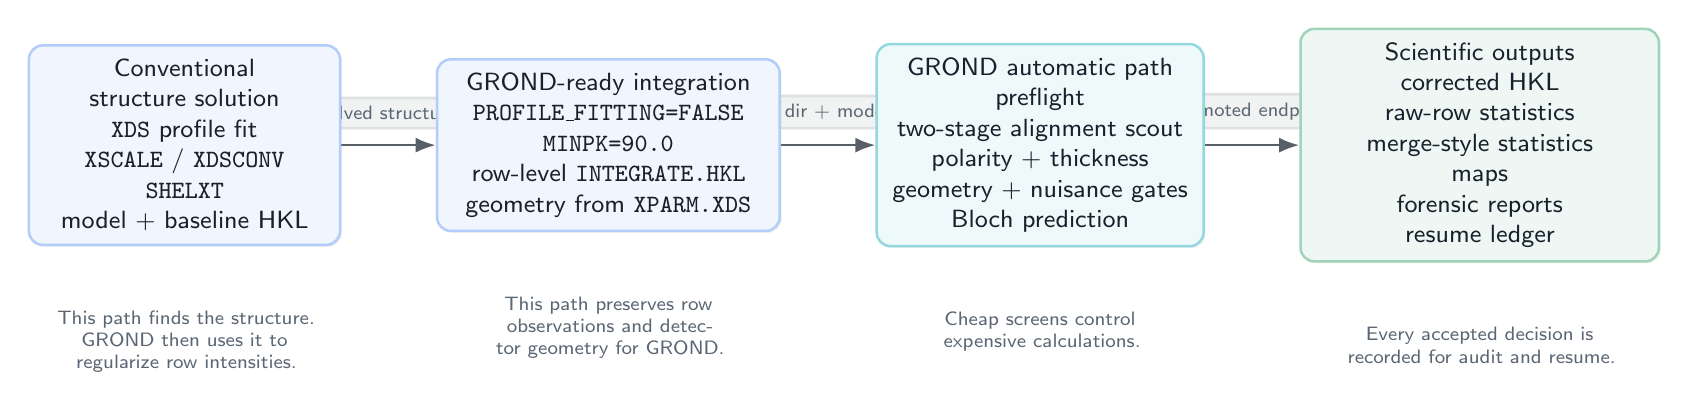
\begin{tikzpicture}[node distance=10mm and 12mm]
  \node[inputbox, text width=36mm] (before) {Conventional structure solution\\
    \texttt{XDS} profile fit\\
    \texttt{XSCALE} / \texttt{XDSCONV}\\
    \texttt{SHELXT}\\
    model + baseline HKL};
  \node[inputbox, text width=40mm, right=of before] (reint) {GROND-ready integration\\
    \texttt{PROFILE\_FITTING=FALSE}\\
    \texttt{MINPK=90.0}\\
    row-level \texttt{INTEGRATE.HKL}\\
    geometry from \texttt{XPARM.XDS}};
  \node[enginebox, text width=38mm, right=of reint] (grond) {GROND automatic path\\
    preflight\\
    two-stage alignment scout\\
    polarity + thickness\\
    geometry + nuisance gates\\
    Bloch prediction};
  \node[outputbox, text width=42mm, right=of grond] (out) {Scientific outputs\\
    corrected HKL\\
    raw-row statistics\\
    merge-style statistics\\
    maps\\
    forensic reports\\
    resume ledger};

  \begin{scope}[on background layer]
    \draw[flow] (before) -- node[tag, above=2mm] {solved structure} (reint);
    \draw[flow] (reint) -- node[tag, above=2mm] {XDS dir + model dir} (grond);
    \draw[flow] (grond) -- node[tag, above=2mm] {promoted endpoint} (out);
  \end{scope}

  \node[note, below=7mm of before, text width=36mm] {This path finds the structure. GROND then uses it to regularize row intensities.};
  \node[note, below=7mm of reint, text width=40mm] {This path preserves row observations and detector geometry for GROND.};
  \node[note, below=7mm of grond, text width=38mm] {Cheap screens control expensive calculations.};
  \node[note, below=7mm of out, text width=42mm] {Every accepted decision is recorded for audit and resume.};
\end{tikzpicture}
}
\caption{High-level GROND flow. The conventional path supplies a chemically sensible starting model; the GROND path starts from row-level integration data and regularizes observed intensities using non-kinematical Bloch/Born predictions.}
\end{figure}

\clearpage

\begin{figure}[p]
\centering
\grondTitle{Before GROND: Conventional Structure-Solution Path}
\grondSub{This is the familiar route used to obtain the starting model and baseline reflection file.}
\resizebox{0.98\linewidth}{!}{%
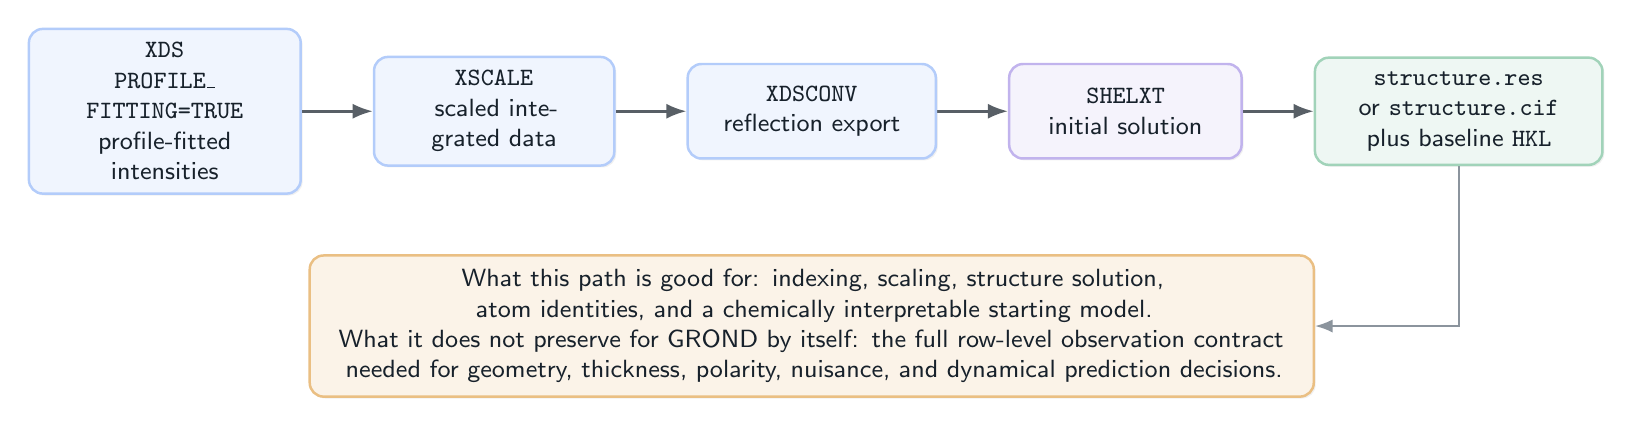
\begin{tikzpicture}[node distance=8mm and 9mm]
  \node[inputbox, text width=31mm] (xds) {\texttt{XDS}\\\texttt{PROFILE\_}\\\texttt{FITTING=TRUE}\\profile-fitted intensities};
  \node[inputbox, text width=27mm, right=of xds] (xscale) {\texttt{XSCALE}\\scaled integrated data};
  \node[inputbox, text width=28mm, right=of xscale] (conv) {\texttt{XDSCONV}\\reflection export};
  \node[updatebox, text width=26mm, right=of conv] (shelxt) {\texttt{SHELXT}\\initial solution};
  \node[outputbox, text width=33mm, right=of shelxt] (model) {\texttt{structure.res}\\or \texttt{structure.cif}\\plus baseline \texttt{HKL}};

  \begin{scope}[on background layer]
    \draw[flow] (xds) -- (xscale);
    \draw[flow] (xscale) -- (conv);
    \draw[flow] (conv) -- (shelxt);
    \draw[flow] (shelxt) -- (model);
  \end{scope}

  \node[riskbox, text width=124mm, below=12mm of conv] (limit) {What this path is good for: indexing, scaling, structure solution, atom identities, and a chemically interpretable starting model.\\
  What it does not preserve for GROND by itself: the full row-level observation contract needed for geometry, thickness, polarity, nuisance, and dynamical prediction decisions.};
  \begin{scope}[on background layer]
    \draw[softflow] (model.south) |- (limit.east);
  \end{scope}
\end{tikzpicture}
}
\caption{The pre-GROND path produces the starting model and baseline HKL. GROND keeps this path as provenance but does not treat it as the final physical model.}
\end{figure}

\clearpage

\begin{figure}[p]
\centering
\grondTitle{After GROND Is Introduced: Reintegrate for Row-Level Physics}
\grondSub{GROND needs the solved structure and a row-preserving XDS directory, not just a merged endpoint.}
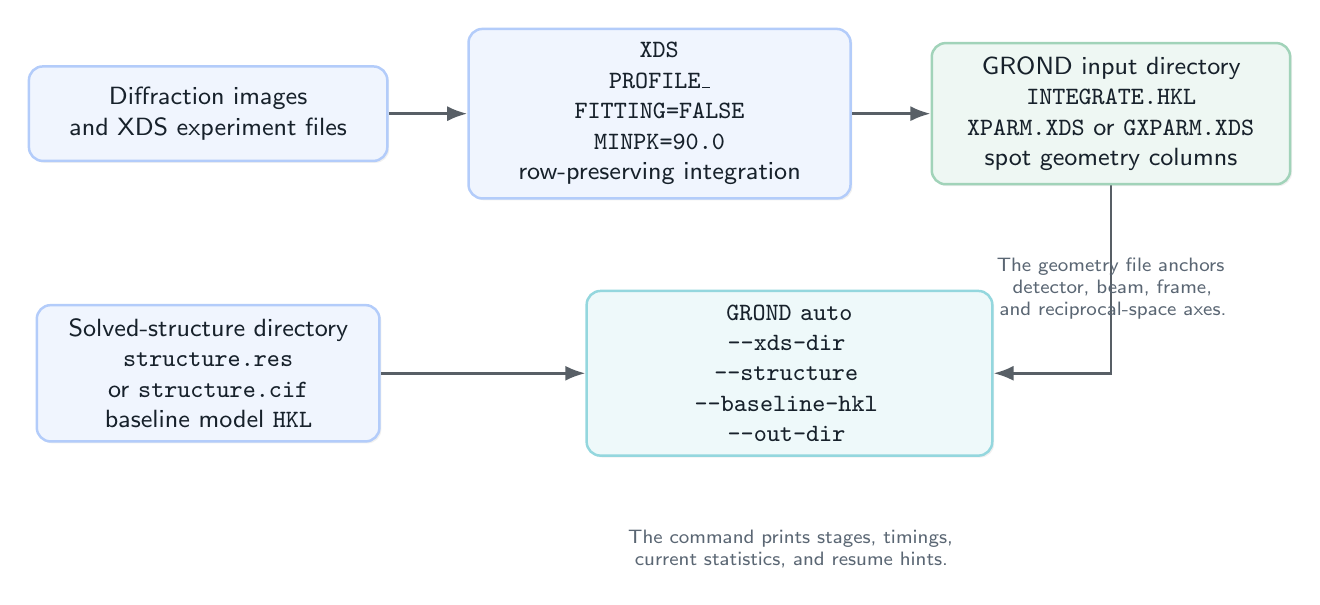
\begin{tikzpicture}[node distance=8mm and 10mm]
  \node[inputbox, text width=42mm] (raw) {Diffraction images\\and XDS experiment files};
  \node[inputbox, text width=45mm, right=of raw] (xds) {\texttt{XDS}\\\texttt{PROFILE\_}\\\texttt{FITTING=FALSE}\\\texttt{MINPK=90.0}\\row-preserving integration};
  \node[outputbox, text width=42mm, right=of xds] (xdsdir) {GROND input directory\\\texttt{INTEGRATE.HKL}\\\texttt{XPARM.XDS} or \texttt{GXPARM.XDS}\\spot geometry columns};

  \node[inputbox, text width=40mm, below=18mm of raw] (structdir) {Solved-structure directory\\\texttt{structure.res} or \texttt{structure.cif}\\baseline model \texttt{HKL}};
  \node[enginebox, text width=48mm, right=26mm of structdir] (feed) {\texttt{GROND auto}\\\texttt{--xds-dir}\\\texttt{--structure}\\\texttt{--baseline-hkl}\\\texttt{--out-dir}};

  \begin{scope}[on background layer]
    \draw[flow] (raw) -- (xds);
    \draw[flow] (xds) -- (xdsdir);
    \draw[flow] (xdsdir.south) |- (feed.east);
    \draw[flow] (structdir) -- (feed);
  \end{scope}

  \node[note, text width=48mm, below=8mm of feed] {The command prints stages, timings, current statistics, and resume hints.};
  \node[note, text width=42mm, below=8mm of xdsdir] {The geometry file anchors detector, beam, frame, and reciprocal-space axes.};
\end{tikzpicture}
\caption{Recommended GROND intake. The row-preserving XDS run provides the observation contract; the solved structure provides the atomic model and baseline reflection alignment.}
\end{figure}

\clearpage

\begin{figure}[p]
\centering
\grondTitle{Stage 1: Observation Intake and Reflection JSON}
\grondSub{GROND converts files into an explicit row ledger before doing expensive physics.}
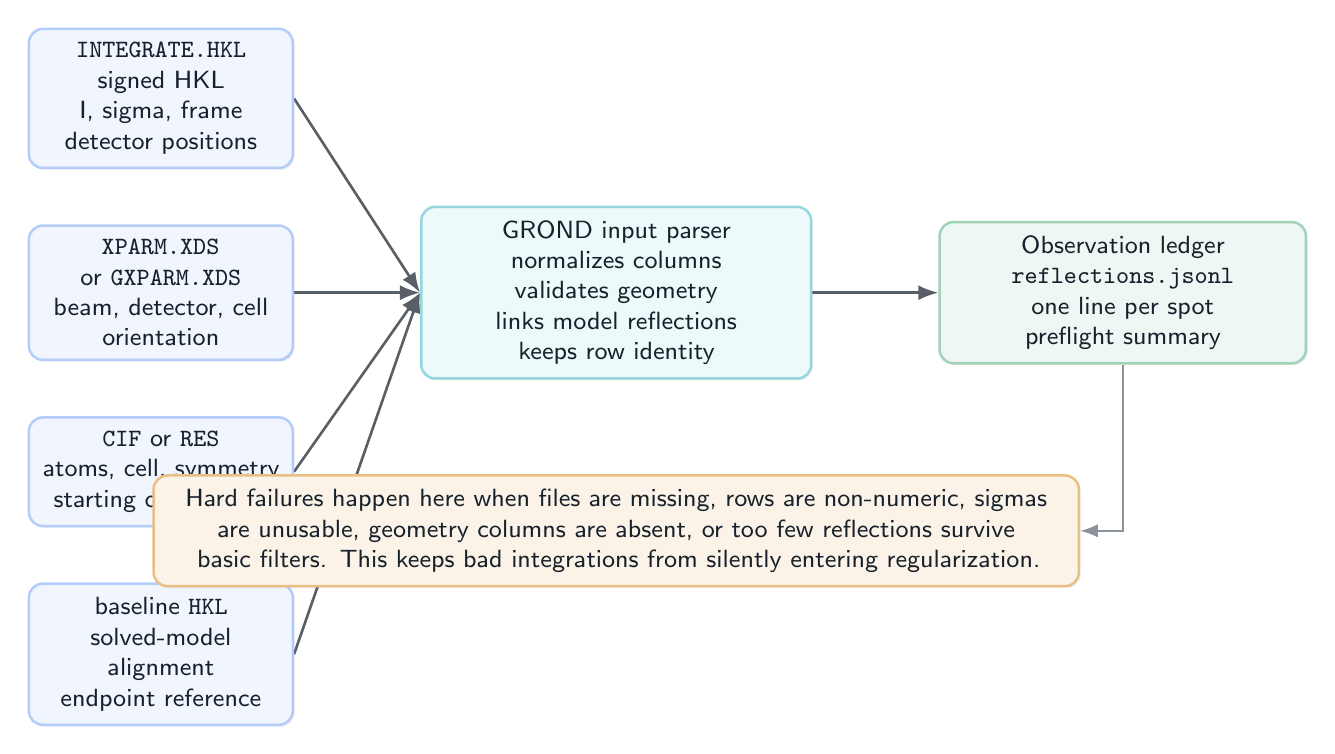
\begin{tikzpicture}[node distance=7mm and 8mm]
  \node[inputbox, text width=30mm] (hkl) {\texttt{INTEGRATE.HKL}\\signed HKL\\I, sigma, frame\\detector positions};
  \node[inputbox, text width=30mm, below=of hkl] (xparm) {\texttt{XPARM.XDS}\\or \texttt{GXPARM.XDS}\\beam, detector, cell\\orientation};
  \node[inputbox, text width=30mm, below=of xparm] (model) {\texttt{CIF} or \texttt{RES}\\atoms, cell, symmetry\\starting coordinates};
  \node[inputbox, text width=30mm, below=of model] (base) {baseline \texttt{HKL}\\solved-model alignment\\endpoint reference};

  \node[enginebox, text width=46mm, right=16mm of xparm] (parser) {GROND input parser\\normalizes columns\\validates geometry\\links model reflections\\keeps row identity};
  \node[outputbox, text width=43mm, right=16mm of parser] (json) {Observation ledger\\\texttt{reflections.jsonl}\\one line per spot\\preflight summary};

  \begin{scope}[on background layer]
    \foreach \a in {hkl,xparm,model,base} {
      \draw[flow] (\a.east) -- (parser.west);
    }
    \draw[flow] (parser) -- (json);
  \end{scope}

  \node[riskbox, text width=114mm, below=12mm of parser] (audit) {Hard failures happen here when files are missing, rows are non-numeric, sigmas are unusable, geometry columns are absent, or too few reflections survive basic filters. This keeps bad integrations from silently entering regularization.};
  \begin{scope}[on background layer]
    \draw[softflow] (json.south) |- (audit.east);
  \end{scope}
\end{tikzpicture}
\caption{Reflection JSON creation. GROND first builds a machine-readable observation ledger so later stages can be audited, resumed, and compared row by row.}
\end{figure}

\clearpage

\begin{figure}[p]
\centering
\grondTitle{Stage 2: Automatic Decision Tree}
\grondSub{GROND avoids a giant blind grid search by making cheap, reversible decisions before expensive final predictions.}
\resizebox{0.98\linewidth}{!}{%
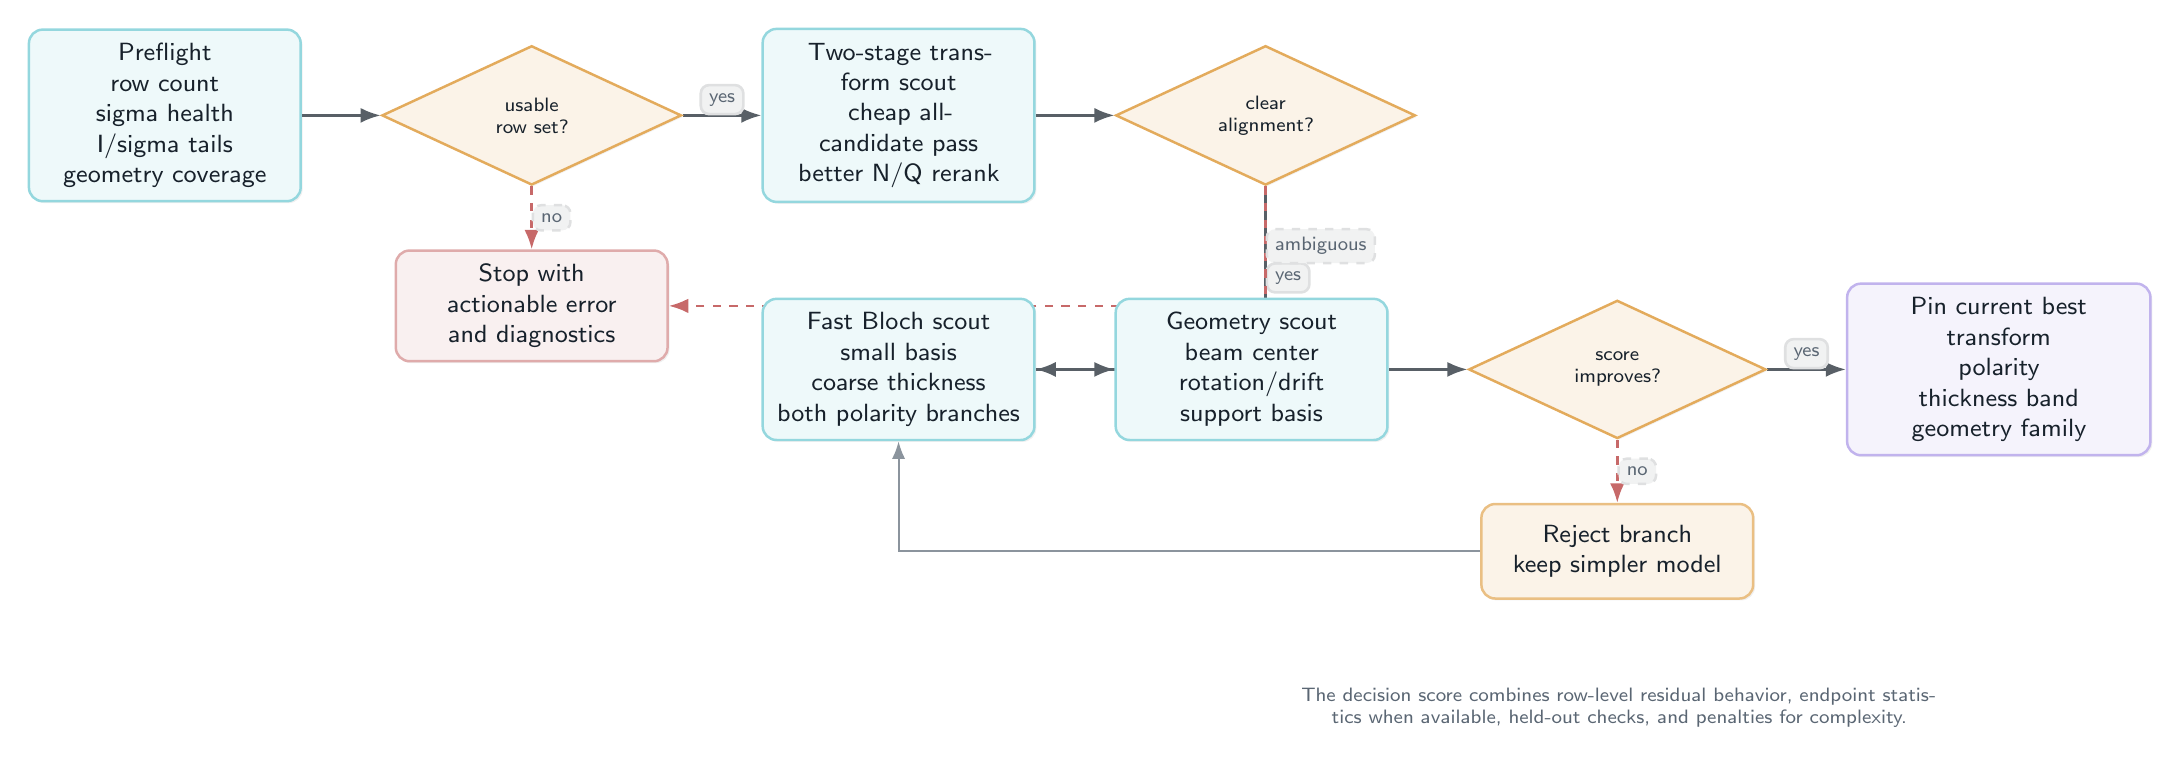
\begin{tikzpicture}[node distance=8mm and 10mm]
  \node[enginebox, text width=31mm] (pre) {Preflight\\row count\\sigma health\\I/sigma tails\\geometry coverage};
  \node[decision, right=of pre, text width=25mm] (usable) {usable\\row set?};
  \node[enginebox, text width=31mm, right=of usable] (transform) {Two-stage transform scout\\cheap all-candidate pass\\better N/Q rerank};
  \node[decision, right=of transform, text width=24mm] (align) {clear\\alignment?};
  \node[enginebox, text width=31mm, below=12mm of transform] (fast) {Fast Bloch scout\\small basis\\coarse thickness\\both polarity branches};
  \node[enginebox, text width=31mm, right=of fast] (geom) {Geometry scout\\beam center\\rotation/drift\\support basis};
  \node[decision, right=of geom, text width=25mm] (promote) {score\\improves?};
  \node[updatebox, text width=35mm, right=of promote] (pin) {Pin current best\\transform\\polarity\\thickness band\\geometry family};
  \node[stopbox, text width=31mm, below=of usable] (stop) {Stop with\\actionable error\\and diagnostics};
  \node[riskbox, text width=31mm, below=of promote] (reject) {Reject branch\\keep simpler model};

  \begin{scope}[on background layer]
    \draw[flow] (pre) -- (usable);
    \draw[flow] (usable) -- node[tag, above] {yes} (transform);
    \draw[rejectflow] (usable) -- node[tag, right] {no} (stop);
    \draw[flow] (transform) -- (align);
    \draw[flow] (align) |- node[tag, pos=0.25, right] {yes} (fast);
    \draw[rejectflow] (align) |- node[tag, pos=0.25, right] {ambiguous} (stop);
    \draw[flow] (fast) -- (geom);
    \draw[flow] (geom) -- (promote);
    \draw[flow] (promote) -- node[tag, above] {yes} (pin);
    \draw[rejectflow] (promote) -- node[tag, right] {no} (reject);
    \draw[softflow] (reject.west) -| (fast.south);
  \end{scope}

  \node[note, text width=126mm, below=10mm of reject] {The decision score combines row-level residual behavior, endpoint statistics when available, held-out checks, and penalties for complexity.};
\end{tikzpicture}
}
\caption{Automatic decision tree. GROND promotes a branch only when it improves the chosen score without creating obvious weak-row, high-resolution, or held-out damage.}
\end{figure}

\clearpage

\begin{figure}[p]
\centering
\grondTitle{Stage 3: Alignment, Geometry, Thickness, and Coordinate polarity}
\grondSub{These are the first physically meaningful parameters GROND must settle before full regularization.}
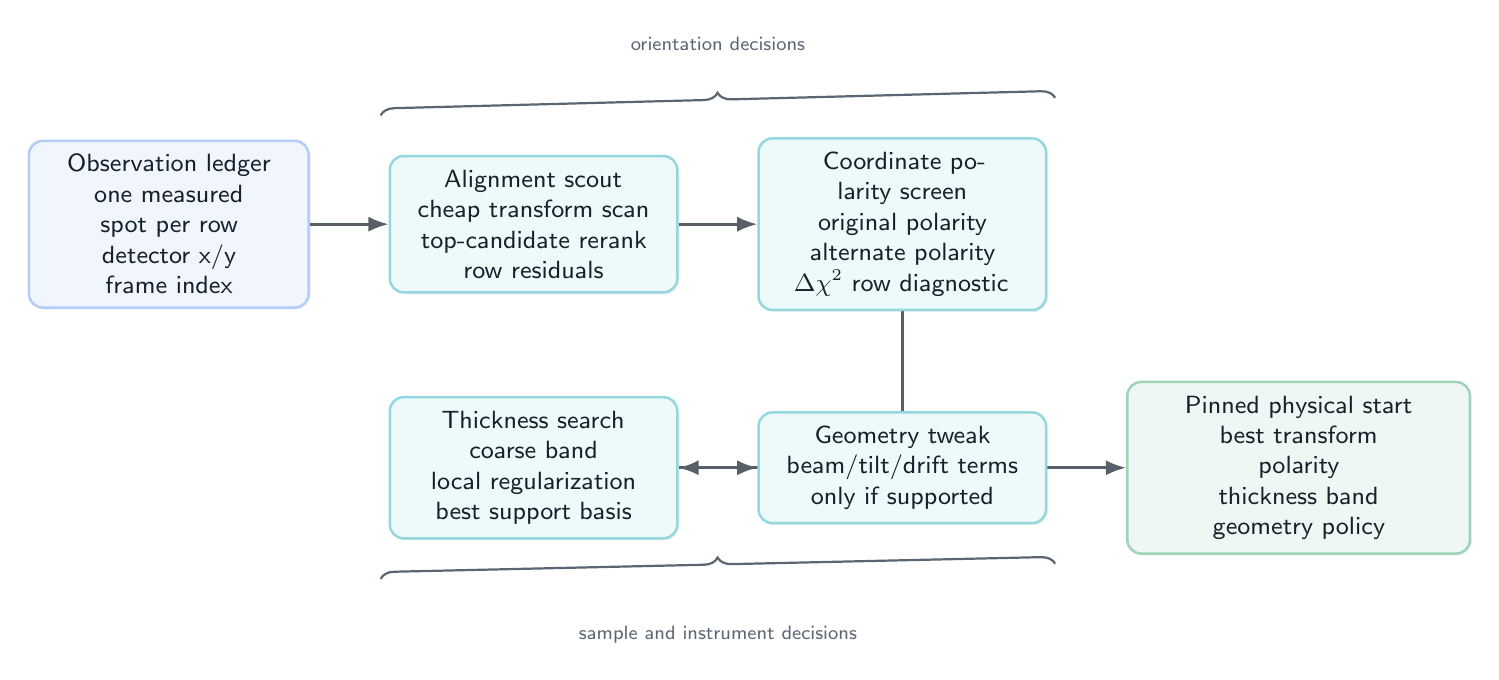
\begin{tikzpicture}[node distance=8mm and 10mm]
  \node[inputbox, text width=32mm] (ledger) {Observation ledger\\one measured spot per row\\detector x/y\\frame index};
  \node[enginebox, text width=33mm, right=of ledger] (align) {Alignment scout\\cheap transform scan\\top-candidate rerank\\row residuals};
  \node[enginebox, text width=33mm, right=of align] (polarity) {Coordinate polarity screen\\original polarity\\alternate polarity\\$\Delta\chi^2$ row diagnostic};
  \node[enginebox, text width=33mm, below=13mm of align] (thick) {Thickness search\\coarse band\\local regularization\\best support basis};
  \node[enginebox, text width=33mm, right=of thick] (geo) {Geometry tweak\\beam/tilt/drift terms\\only if supported};
  \node[outputbox, text width=40mm, right=of geo] (pinned) {Pinned physical start\\best transform\\polarity\\thickness band\\geometry policy};

  \begin{scope}[on background layer]
    \draw[flow] (ledger) -- (align);
    \draw[flow] (align) -- (polarity);
    \draw[flow] (polarity) |- (thick);
    \draw[flow] (thick) -- (geo);
    \draw[flow] (geo) -- (pinned);
  \end{scope}

  \draw[decorate, decoration={brace, amplitude=5pt}, thick, draw=grondMuted]
    ($(align.north west)+(-1mm,5mm)$) -- ($(polarity.north east)+(1mm,5mm)$)
    node[midway, yshift=8mm, note] {orientation decisions};
  \draw[decorate, decoration={brace, amplitude=5pt}, thick, draw=grondMuted]
    ($(thick.south west)+(-1mm,-5mm)$) -- ($(geo.south east)+(1mm,-5mm)$)
    node[midway, yshift=-8mm, note] {sample and instrument decisions};
\end{tikzpicture}
\caption{Early physical decisions. The goal is not to test every possible setting, but to find a stable transform, polarity, thickness band, and geometry family quickly enough to make the final regularization tractable.}
\end{figure}

\clearpage

\begin{figure}[p]
\centering
\grondTitle{Stage 4: Bloch Prediction and Intensity Regularization}
\grondSub{The central loop simulates Bloch and Born row intensities, regularizes measured observations, and updates only supported non-scattering terms.}
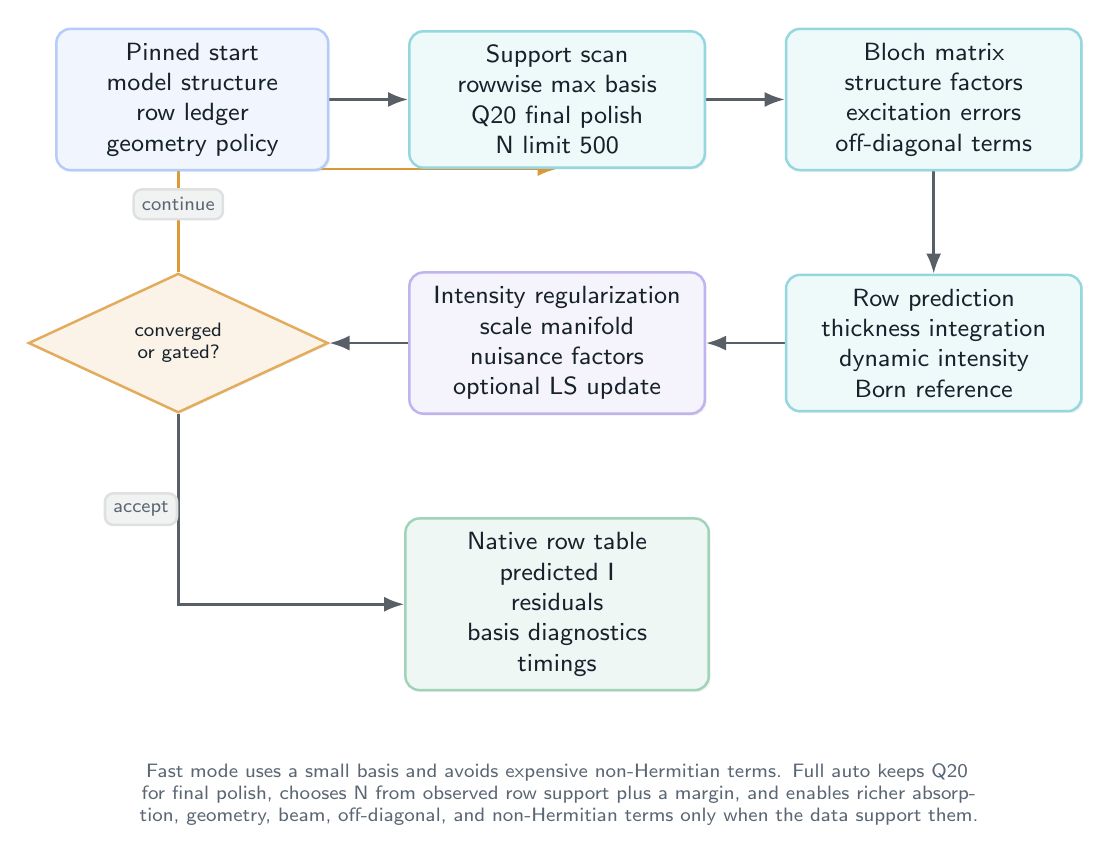
\begin{tikzpicture}[node distance=8mm and 10mm]
  \node[inputbox, text width=31mm] (start) {Pinned start\\model structure\\row ledger\\geometry policy};
  \node[enginebox, text width=34mm, right=of start] (basis) {Support scan\\rowwise max basis\\Q20 final polish\\N limit 500};
  \node[enginebox, text width=34mm, right=of basis] (matrix) {Bloch matrix\\structure factors\\excitation errors\\off-diagonal terms};
  \node[enginebox, text width=34mm, below=13mm of matrix] (predict) {Row prediction\\thickness integration\\dynamic intensity\\Born reference};
  \node[updatebox, text width=34mm, left=of predict] (regularize) {Intensity regularization\\scale manifold\\nuisance factors\\optional LS update};
  \node[decision, left=of regularize, text width=24mm] (conv) {converged\\or gated?};
  \node[outputbox, text width=35mm, below=13mm of regularize] (rows) {Native row table\\predicted I\\residuals\\basis diagnostics\\timings};

  \begin{scope}[on background layer]
    \draw[flow] (start) -- (basis);
    \draw[flow] (basis) -- (matrix);
    \draw[flow] (matrix) -- (predict);
    \draw[flow] (predict) -- (regularize);
    \draw[flow] (regularize) -- (conv);
    \draw[gateflow] (conv.north) |- node[tag, pos=0.25, above] {continue} (basis.south);
    \draw[flow] (conv) |- node[tag, pos=0.25, left] {accept} (rows);
  \end{scope}

  \node[note, text width=118mm, below=8mm of rows] {Fast mode uses a small basis and avoids expensive non-Hermitian terms. Full auto keeps Q20 for final polish, chooses N from observed row support plus a margin, and enables richer absorption, geometry, beam, off-diagonal, and non-Hermitian terms only when the data support them.};
\end{tikzpicture}
\caption{Bloch/regularization core. GROND separates cheap scouting from the final high-fidelity prediction so runtime is spent on branches that have already earned promotion.}
\end{figure}

\clearpage

\begin{figure}[p]
\centering
\grondTitle{Stage 5: Nuisance Terms, Forensics, and Promotion Gates}
\grondSub{GROND treats nuisance terms as hypotheses that must improve held-out behavior, not as automatic curve-fit knobs.}
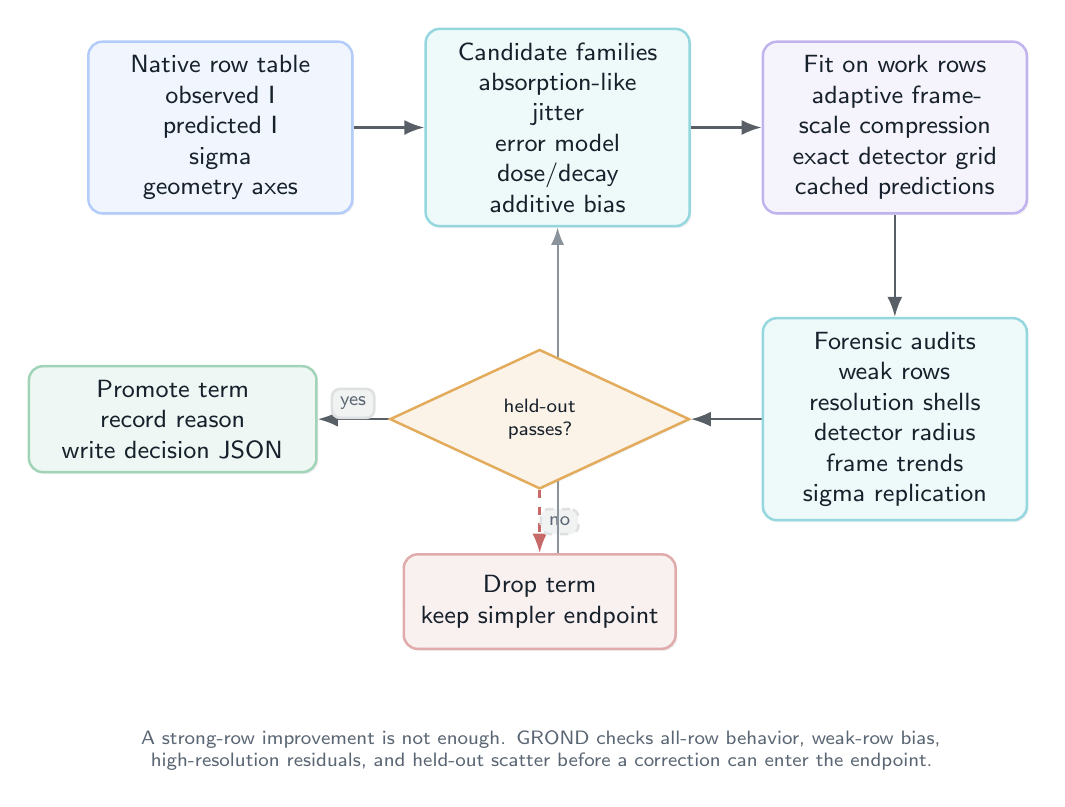
\begin{tikzpicture}[node distance=8mm and 9mm]
  \node[inputbox, text width=30mm] (rows) {Native row table\\observed I\\predicted I\\sigma\\geometry axes};
  \node[enginebox, text width=30mm, right=of rows] (families) {Candidate families\\absorption-like\\jitter\\error model\\dose/decay\\additive bias};
  \node[updatebox, text width=30mm, right=of families] (fit) {Fit on work rows\\adaptive frame-scale compression\\exact detector grid\\cached predictions};
  \node[enginebox, text width=30mm, below=13mm of fit] (audit) {Forensic audits\\weak rows\\resolution shells\\detector radius\\frame trends\\sigma replication};
  \node[decision, text width=24mm, left=of audit] (gate) {held-out\\passes?};
  \node[outputbox, text width=33mm, left=of gate] (promote) {Promote term\\record reason\\write decision JSON};
  \node[stopbox, text width=31mm, below=of gate] (drop) {Drop term\\keep simpler endpoint};

  \begin{scope}[on background layer]
    \draw[flow] (rows) -- (families);
    \draw[flow] (families) -- (fit);
    \draw[flow] (fit) -- (audit);
    \draw[flow] (audit) -- (gate);
    \draw[flow] (gate) -- node[tag, above] {yes} (promote);
    \draw[rejectflow] (gate) -- node[tag, right] {no} (drop);
    \draw[softflow] (drop.west) -| (families.south);
  \end{scope}

  \node[note, text width=124mm, below=9mm of drop] {A strong-row improvement is not enough. GROND checks all-row behavior, weak-row bias, high-resolution residuals, and held-out scatter before a correction can enter the endpoint.};
\end{tikzpicture}
\caption{Nuisance and forensic gatekeeping. The package promotes only terms that improve the physical model without hiding failures in scale factors or weak reflections.}
\end{figure}

\clearpage

\begin{figure}[p]
\centering
\grondTitle{Stage 6: Endpoint Files, Maps, and Resume Ledger}
\grondSub{Every run ends with auditable artifacts, even when optional external map or regularization programs are absent.}
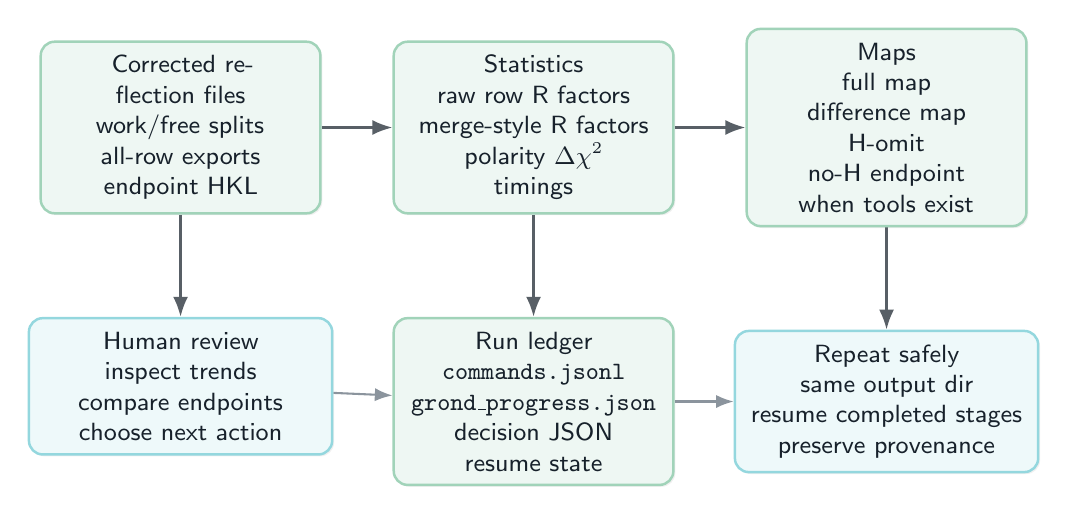
\begin{tikzpicture}[node distance=8mm and 9mm]
  \node[outputbox, text width=32mm] (corr) {Corrected reflection files\\work/free splits\\all-row exports\\endpoint HKL};
  \node[outputbox, text width=32mm, right=of corr] (stats) {Statistics\\raw row R factors\\merge-style R factors\\polarity $\Delta\chi^2$\\timings};
  \node[outputbox, text width=32mm, right=of stats] (maps) {Maps\\full map\\difference map\\H-omit\\no-H endpoint\\when tools exist};
  \node[outputbox, text width=32mm, below=13mm of stats] (ledger) {Run ledger\\\texttt{commands.jsonl}\\\texttt{grond\_progress.json}\\decision JSON\\resume state};
  \node[enginebox, text width=35mm, below=13mm of corr] (user) {Human review\\inspect trends\\compare endpoints\\choose next action};
  \node[enginebox, text width=35mm, below=13mm of maps] (repeat) {Repeat safely\\same output dir\\resume completed stages\\preserve provenance};

  \begin{scope}[on background layer]
    \draw[flow] (corr) -- (stats);
    \draw[flow] (stats) -- (maps);
    \draw[flow] (corr) -- (user);
    \draw[flow] (stats) -- (ledger);
    \draw[flow] (maps) -- (repeat);
    \draw[softflow] (ledger) -- (repeat);
    \draw[softflow] (user) -- (ledger);
  \end{scope}
\end{tikzpicture}
\caption{Endpoint and artifact production. GROND produces corrected reflection files, statistics, maps when possible, and a resume ledger so interrupted runs can continue without losing provenance.}
\end{figure}

\clearpage

\begin{figure}[p]
\centering
\grondTitle{Multi-Dataset Prep File Workflow}
\grondSub{One solved structure can drive several XDS directories while keeping dataset-specific decisions separate.}
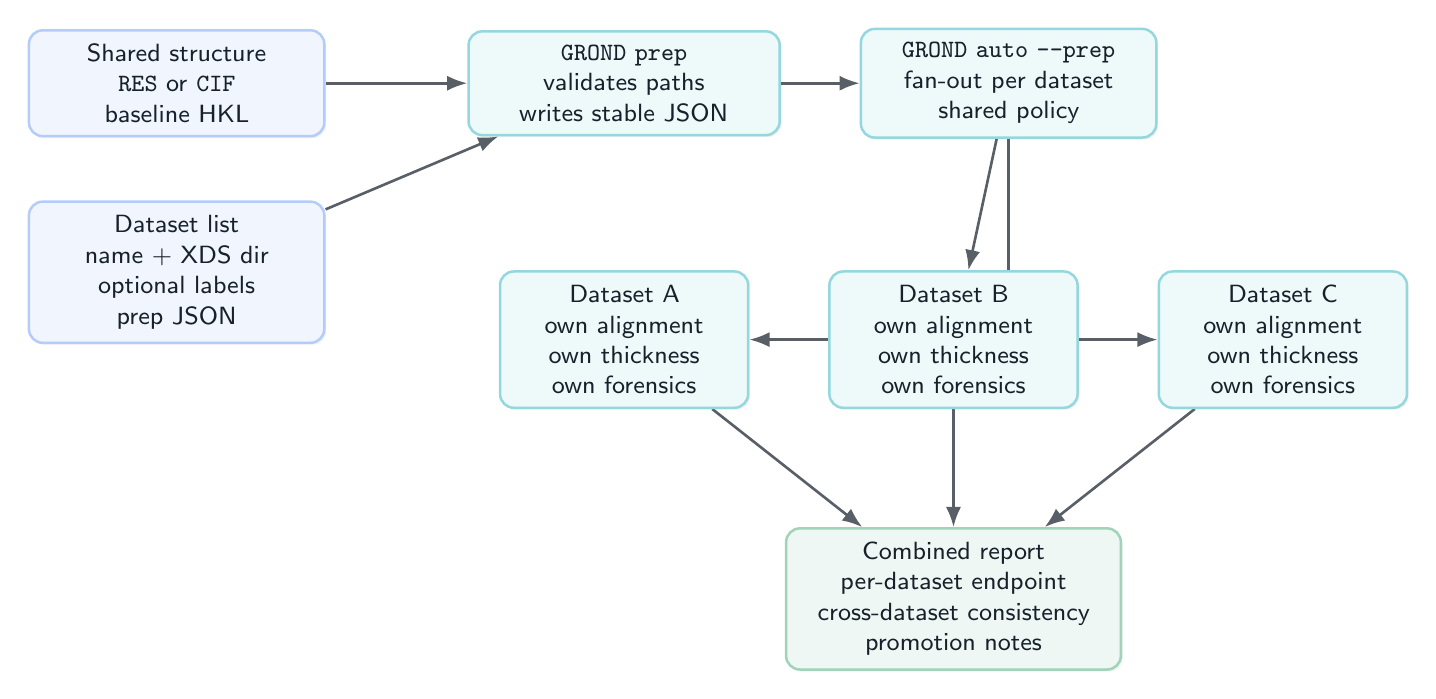
\begin{tikzpicture}[node distance=8mm and 10mm]
  \node[inputbox, text width=34mm] (struct) {Shared structure\\\texttt{RES} or \texttt{CIF}\\baseline HKL};
  \node[inputbox, text width=34mm, below=of struct] (list) {Dataset list\\name + XDS dir\\optional labels\\prep JSON};
  \node[enginebox, text width=36mm, right=18mm of struct] (prep) {\texttt{GROND prep}\\validates paths\\writes stable JSON};
  \node[enginebox, text width=34mm, right=of prep] (fan) {\texttt{GROND auto --prep}\\fan-out per dataset\\shared policy};

  \node[enginebox, text width=28mm, below=17mm of prep] (d1) {Dataset A\\own alignment\\own thickness\\own forensics};
  \node[enginebox, text width=28mm, right=of d1] (d2) {Dataset B\\own alignment\\own thickness\\own forensics};
  \node[enginebox, text width=28mm, right=of d2] (d3) {Dataset C\\own alignment\\own thickness\\own forensics};
  \node[outputbox, text width=39mm, below=15mm of d2] (summary) {Combined report\\per-dataset endpoint\\cross-dataset consistency\\promotion notes};

  \begin{scope}[on background layer]
    \draw[flow] (struct) -- (prep);
    \draw[flow] (list) -- (prep);
    \draw[flow] (prep) -- (fan);
    \draw[flow] (fan) |- (d1);
    \draw[flow] (fan) -- (d2);
    \draw[flow] (fan) |- (d3);
    \draw[flow] (d1) -- (summary);
    \draw[flow] (d2) -- (summary);
    \draw[flow] (d3) -- (summary);
  \end{scope}
\end{tikzpicture}
\caption{Multi-dataset execution. The prep file is a compact manifest: shared structure and baseline model information plus multiple row-preserving XDS directories.}
\end{figure}

\clearpage

\begin{figure}[p]
\centering
\grondTitle{Run Modes and Relative Cost}
\grondSub{The modes expose the same science at different levels of speed, automation, and endpoint ambition. The chart is qualitative, not a benchmark.}
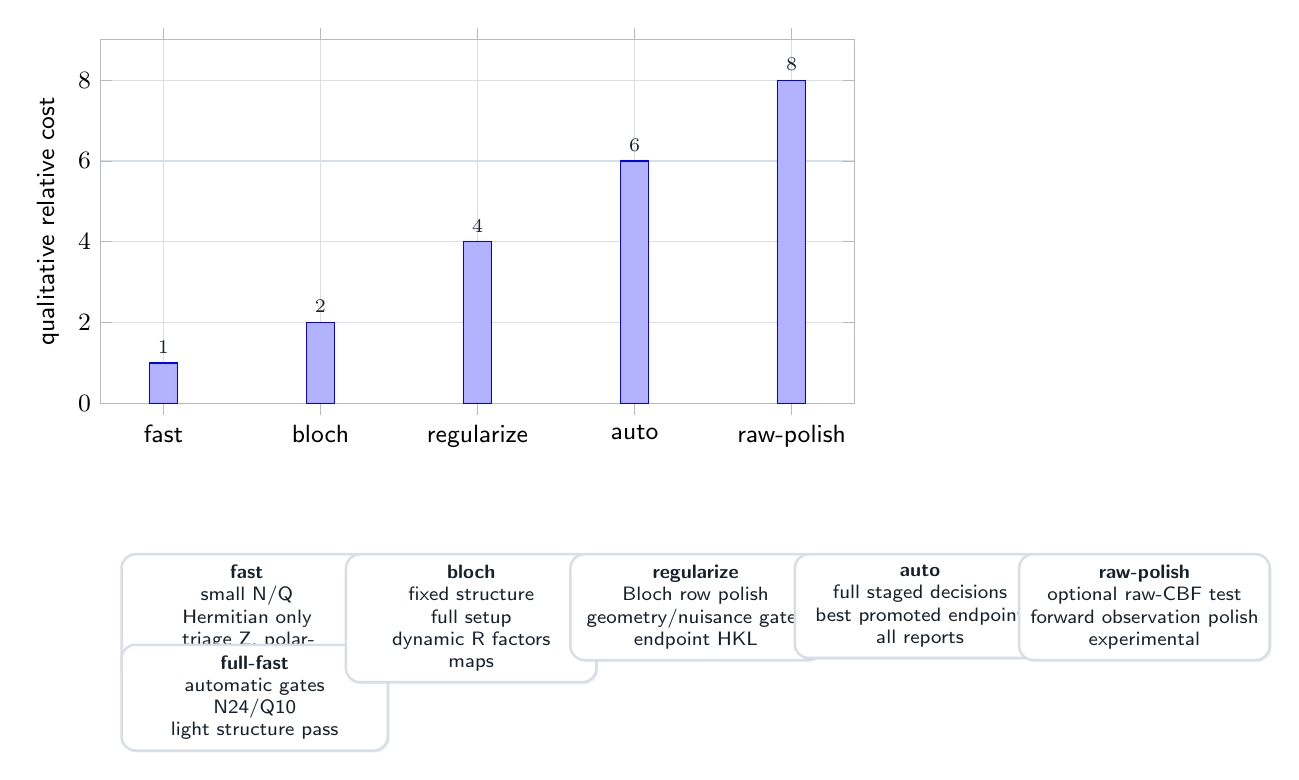
\begin{tikzpicture}
  \begin{axis}[
    width=0.92\linewidth,
    height=62mm,
    ybar,
    bar width=10pt,
    ymin=0,
    ymax=9,
    ylabel={qualitative relative cost},
    symbolic x coords={fast,bloch,regularize,auto,raw-polish},
    xtick=data,
    x tick label style={font=\sffamily\small},
    y tick label style={font=\sffamily\small},
    ylabel style={font=\sffamily\small},
    axis line style={draw=grondMuted!45},
    tick style={draw=grondMuted!45},
    grid=major,
    grid style={draw=grondLine},
    nodes near coords,
    nodes near coords style={font=\sffamily\scriptsize, text=grondInk},
    every axis plot/.append style={fill=grondBlue!55, draw=grondBlue!75}
  ]
    \addplot coordinates {(fast,1) (bloch,2) (regularize,4) (auto,6) (raw-polish,8)};
  \end{axis}

  \node[smallbox, text width=29mm, anchor=north west] at (0.25,-1.9) {\textbf{fast}\\small N/Q\\Hermitian only\\triage Z, polarity, thickness};
  \node[smallbox, text width=31mm, anchor=north west] at (0.25,-3.05) {\textbf{full-fast}\\automatic gates\\N24/Q10\\light structure pass};
  \node[smallbox, text width=29mm, anchor=north west] at (3.1,-1.9) {\textbf{bloch}\\fixed structure\\full setup\\dynamic R factors\\maps};
  \node[smallbox, text width=29mm, anchor=north west] at (5.95,-1.9) {\textbf{regularize}\\Bloch row polish\\geometry/nuisance gates\\endpoint HKL};
  \node[smallbox, text width=29mm, anchor=north west] at (8.8,-1.9) {\textbf{auto}\\full staged decisions\\best promoted endpoint\\all reports};
  \node[smallbox, text width=29mm, anchor=north west] at (11.65,-1.9) {\textbf{raw-polish}\\optional raw-CBF test\\forward observation polish\\experimental};
\end{tikzpicture}
\caption{Mode chart. Fast mode is for immediate sanity checks; auto mode is the default walk-away path; raw-polish remains an optional final test layer when raw images and calibration are available.}
\end{figure}

\end{document}
